\documentclass[12pt]{article}

%% Language and font encodings
\usepackage[english]{babel}
\usepackage[utf8x]{inputenc}
\usepackage[T1]{fontenc}
\usepackage{fancyhdr}

%% Sets page size and margins
\usepackage[a4paper,top=3cm,bottom=2cm,left=3cm,right=3cm,marginparwidth=1.75cm]{geometry}

%% Packages
\usepackage{xcolor}
\usepackage[colorlinks=true, allcolors=red]{hyperref}
\usepackage{lipsum}
\usepackage{graphicx}
\usepackage{float}
\usepackage[all]{hypcap}
\usepackage{changepage}
\usepackage{amsmath}
\usepackage{amssymb}
\usepackage{xspace}
\usepackage{tikz}

%% Other
\graphicspath{{Figures/}}
\setlength\parindent{0pt}
\newcommand{\auth}{Giulia Baldini, Luis Fernandes, Agustin Vargas}
\newcommand{\ass}{Assignment 1}

%% Page settings
\pagestyle{fancy}
\fancyhf{}
\rhead{\auth}
\lhead{\ass}
\rfoot{\thepage}

\title{Foundations of Audio Signal Processing\\ \ass}
\author{\auth}

\begin{document}
	\maketitle
	\section*{Exercise 2.1}
	\textbf{a.}
	\begin{alignat*}{3}
		2e^{\frac{\pi}{2} i} (1 + i) &= 2 (\cos(\frac{\pi}{2}) + i\sin(\frac{\pi}{2}))(1 + i)\\
		&= 2i (1 + i)\\
		&= -2 + 2i\\
		a &= -2\\
		b &= 2\\
		r &= \sqrt{(-2)^2 + (2)^2}\\
		&= 2\sqrt{2}\\ 
	\end{alignat*}
	Knowing that $a = \cos(\phi)$ and $b = \sin(\phi)$:
	\begin{alignat*}{3}
	\cos(\phi) &= \frac{-2}{2\sqrt{2}} &= -\frac{\sqrt{2}}{2}\\
	\sin(\phi) &= \frac{2}{2\sqrt{2}} &= \frac{\sqrt{2}}{2}\\
	\phi &= \frac{3}{4}\pi\\
	z &= 2 \sqrt{2} e^{\frac{3}{4}\pi i}
	\end{alignat*}
	\textbf{b.} Considering that $z = re^{\phi i}$, $\overline{z} = re^{-\phi i}$ and $|z| = r$
	\begin{alignat*}{3}
	z \overline{z} &= re^{\phi i} re^{- \phi i}\\
	&= r^2 e^0 &= |z|^2\\
	\end{alignat*}
	\textbf{c.}
	\begin{alignat*}{3}
	\frac{1}{2i} (e^{ia} - e^{-ia}) &= \frac{1}{2i} (\cos(a) + i \sin(a) - (\cos(-a) + i \sin(-a)))\\
	&= \frac{1}{2i} (\cos(a) + i \sin(a) - \cos(a) + i \sin(a))\\
	&= \frac{1}{2i} (2 i \sin(a)) &= \sin(a)
	\end{alignat*}
	\section*{Exercise 2.2}
	\textbf{a.}
	For $n = 4$:
	\begin{alignat*}{2}
	\Omega^1_4 &= \cos(\frac{\pi}{2}) + i \sin (\frac{\pi}{2}) = i\\
	\Omega^2_4 &= \cos(\pi) + i \sin (\pi) = -1\\
	\Omega^3_4 &= \cos(3\frac{\pi}{2}) + i \sin (3\frac{\pi}{2}) = -i\\
	\Omega^4_4 &= 1
	\end{alignat*}
	So the fourth roots of unity are ${1, -1, i, -i}$ and, since 4 is the smallest integer for which $\Omega = {i, -i}$, then these are its primitives.
	\begin{figure}[H]
	\def\n{4}
	\centering
	\begin{tikzpicture}[
	dot/.style={draw,fill,circle,inner sep=1pt}
	]
	\draw[->] (-2,0) -- (2,0) node[below] {$\Re$};
	\draw[->] (0,-2) -- (0,2) node[left] {$\Im$};
	\draw[help lines] (0,0) circle (1);
	
	\node[dot,label={below right:$O$}] (O) at (0,0) {};
	\foreach \i in {1,...,\n} {
		\node[dot,label={\i*360/\n-(\i==\n)*45:$w_{\i}$}] (w\i) at (\i*360/\n:1) {};
		\draw[->] (O) -- (w\i);
	}
	\draw[->] (0:.3) arc (0:360/\n:.3);
	\node at (360/\n/2:.5) {$\alpha$};
	\end{tikzpicture}
	\caption{Illustration of all fourth roots of unity.}
	\end{figure}
	For $n = 6$:
	\begin{alignat*}{2}
	\Omega^1_6 &= \cos(\frac{\pi}{3}) + i \sin (\frac{\pi}{3}) = \frac{1}{2} + \frac{\sqrt{3}}{2}i\\
	\Omega^2_6 &= \cos(2\frac{\pi}{3}) + i \sin (2\frac{\pi}{3}) = - \frac{1}{2} + \frac{\sqrt{3}}{2}i\\
	\Omega^3_6 &= \cos(\pi) + i \sin (\pi) = -1\\
	\Omega^4_6 &= \cos(4\frac{\pi}{3}) + i \sin (4\frac{\pi}{3}) = - \frac{1}{2} - \frac{\sqrt{3}}{2}i\\
	\Omega^5_6 &= \cos(5\frac{\pi}{3}) + i \sin (5\frac{\pi}{3}) = \frac{1}{2} - \frac{\sqrt{3}}{2}i\\
	\Omega^6_6 &= 1
	\end{alignat*}
	So the sixth roots of unity are ${1, -1, \frac{1}{2} + \frac{\sqrt{3}}{2}i, \frac{1}{2} - \frac{\sqrt{3}}{2}i, -\frac{1}{2} - \frac{\sqrt{3}}{2}i, \frac{1}{2} - \frac{\sqrt{3}}{2}i}$ and, since 4 is the smallest integer for which $\Omega = {- \frac{1}{2} + \frac{\sqrt{3}}{2}i, \frac{1}{2} + \frac{\sqrt{3}}{2}i}$, then these are its primitives.\\
	\begin{figure}[H]
	\def\n{6}
	\centering
	\begin{tikzpicture}[
	dot/.style={draw,fill,circle,inner sep=1pt}
	]
	\draw[->] (-2,0) -- (2,0) node[below] {$\Re$};
	\draw[->] (0,-2) -- (0,2) node[left] {$\Im$};
	\draw[help lines] (0,0) circle (1);
	
	\node[dot,label={below right:$O$}] (O) at (0,0) {};
	\foreach \i in {1,...,\n} {
		\node[dot,label={\i*360/\n-(\i==\n)*45:$w_{\i}$}] (w\i) at (\i*360/\n:1) {};
		\draw[->] (O) -- (w\i);
	}
	\draw[->] (0:.3) arc (0:360/\n:.3);
	\node at (360/\n/2:.5) {$\alpha$};
	\end{tikzpicture}
	\caption{Illustration of all sixth roots of unity.}
	\end{figure}
	\textbf{b.} By definition of roots of unity
	\begin{alignat*}{2}
		\sum_{k = 0}^{n-1}\Omega_k &= \omega^0 + \omega^1 + \cdots + \omega^{n-1}
	\end{alignat*}
	where $\omega^k = e^{\frac{2 k \pi i}{n}}$. Since $\omega^0 = 1$, we can write the definition as a finite geometric series
	\begin{alignat*}{2}
	\sum_{k = 0}^{n-1} e^{\frac{2 k \pi i}{n}}&= \frac{1 - e^{\frac{2 n \pi i}{n}}}{1 - e^{\frac{2\pi i}{n}}}
	\end{alignat*}
	since $e^{\frac{2 n \pi i}{n}} = 1$, then 
	\begin{alignat*}{3}
	\sum_{k = 0}^{n-1} \Omega_k &= \frac{0}{1 - e^{\frac{2\pi i}{n}}} &= 0
	\end{alignat*}
	\section*{Exercise 2.3}
	\textbf{a-c.} The solutions can be found inside the \texttt{code} folder.
	\begin{figure}[H]
	\label{plot}
	\centering
	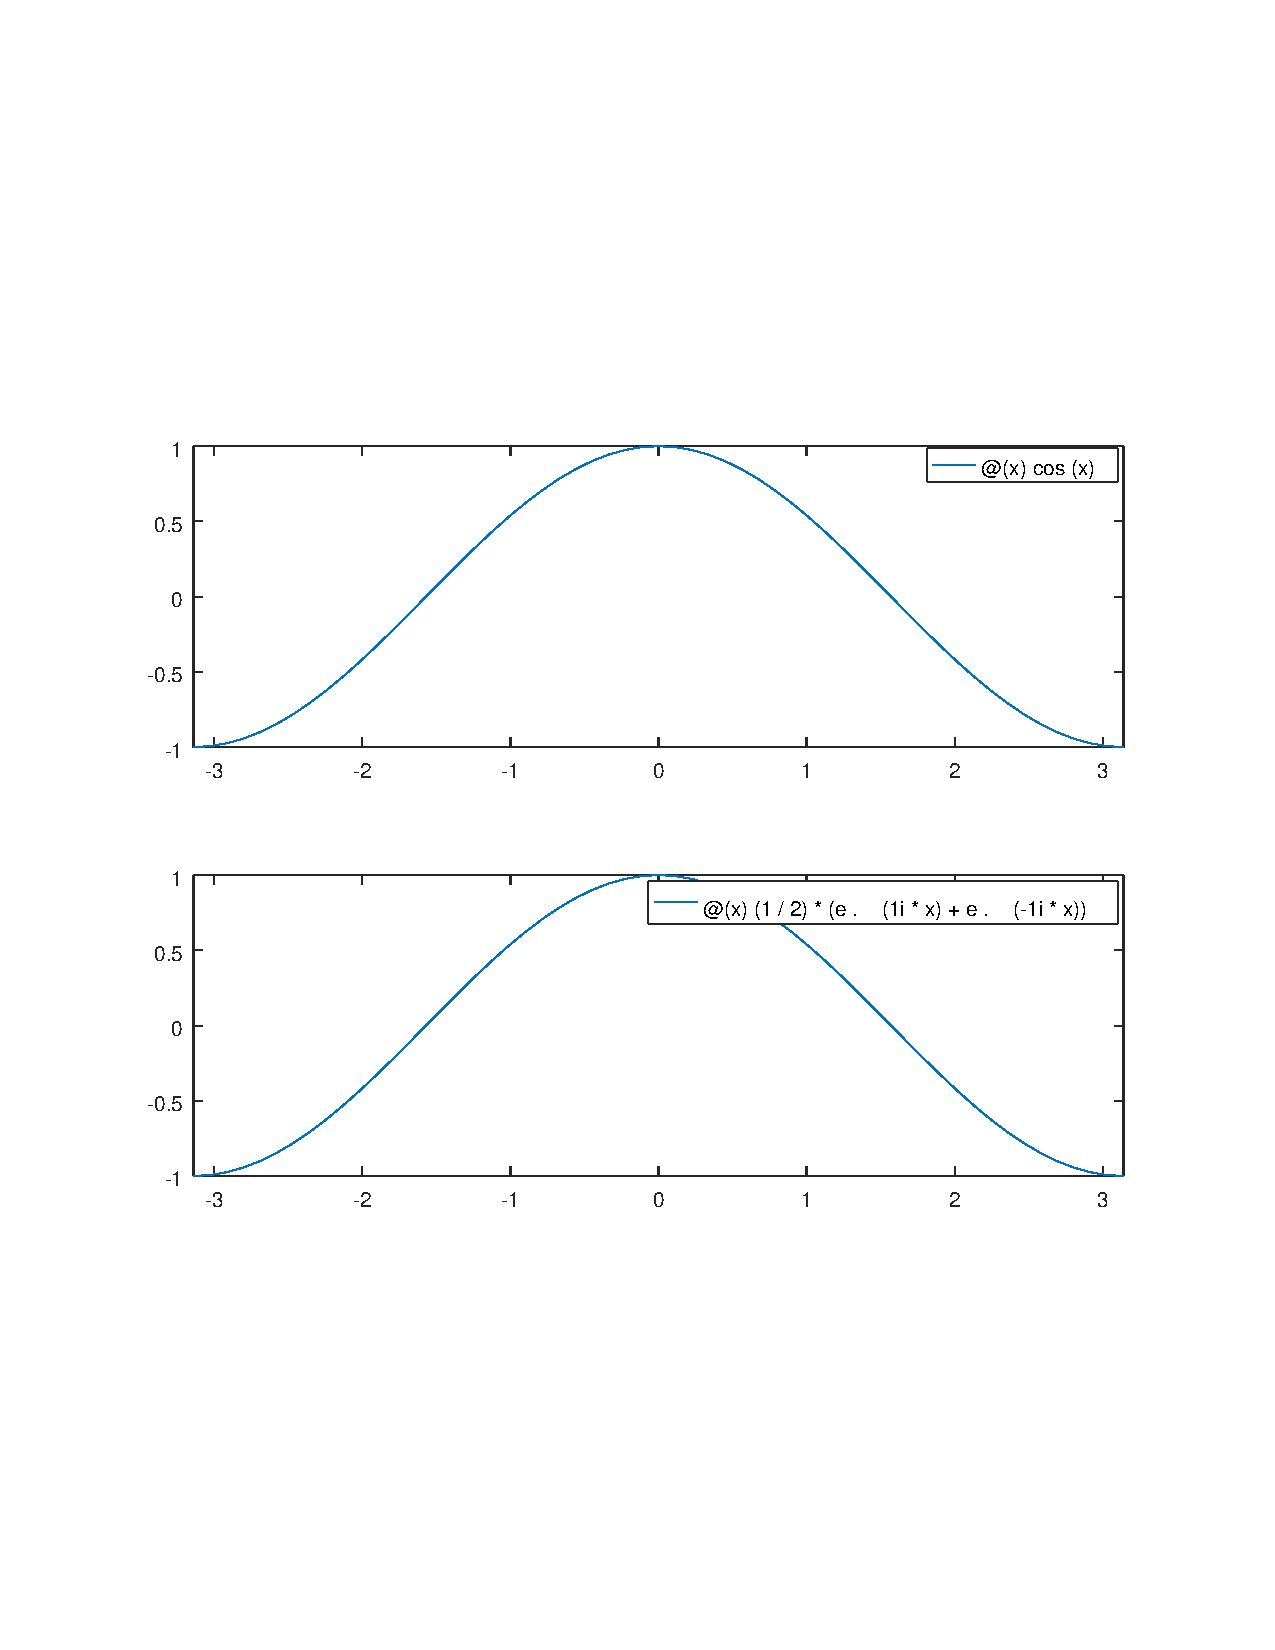
\includegraphics[width=27em]{3c.pdf}
	\caption{Visualization of the statement $\cos(\alpha) = \frac{1}{2} \cdot (e^{i\alpha} + e^{-i\alpha})$ }
	\end{figure}

\end{document}
